% The problem picture and the four steps: page 1 of TLDR.tex and the figure at the top of the README (overview.tex)
% ---------------- the problem in one picture
\node[anchor=north west, font=\bfseries\normalsize] at (0,-0.85) {What you have: many runs on a parameter grid};
\node[anchor=north west, inner sep=0] at (0,-1.4) {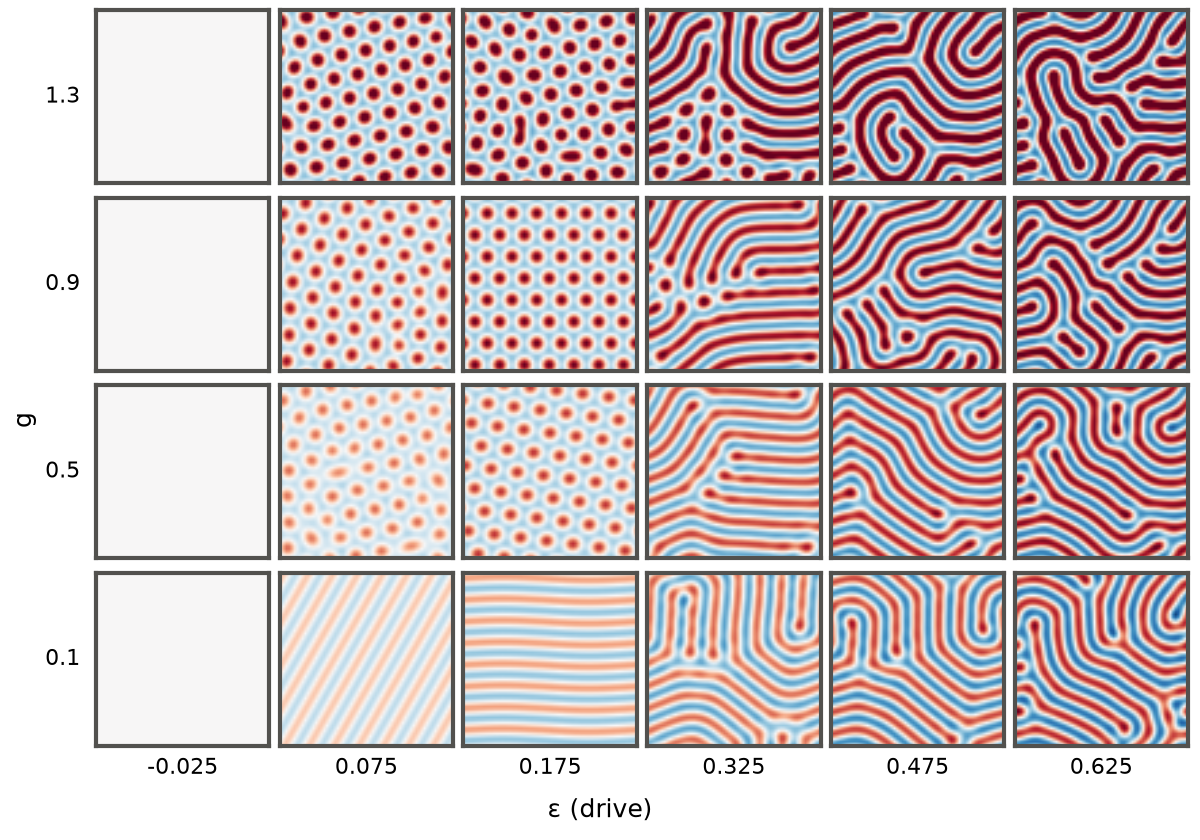
\includegraphics[height=6.6cm]{fig_sh_grid.png}};
\draw[big] (9.75,-4.6) -- (11.65,-4.6);
\node[font=\bfseries\small, align=center] at (10.7,-4.0) {PhaseWall};
\node[font=\footnotesize, align=center] at (10.7,-5.2) {no labels\\no number\\of phases};
\node[anchor=north west, font=\bfseries\normalsize] at (11.8,-0.85) {What you get: phases and walls};
\node[anchor=north west, inner sep=0] at (11.8,-1.25) {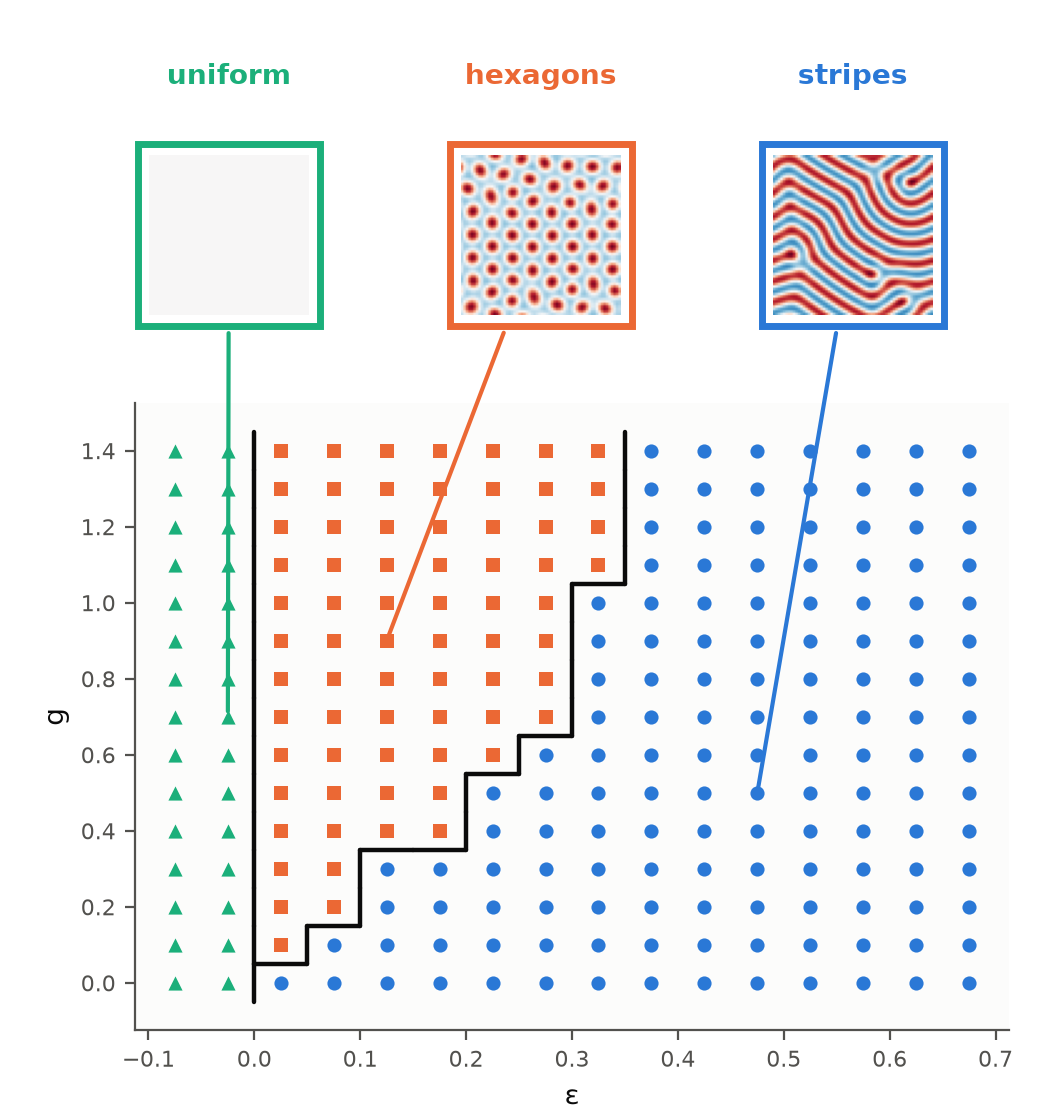
\includegraphics[height=7.0cm]{fig_sh_phases.png}};
\node[say, text width=8.3cm] at (19.6,-1.5) {
\textbf{Example: Swift-Hohenberg}, a model of pattern formation\\[2pt]
$\partial_t u=\varepsilon u-(1+\nabla^2)^2u+g\,u^2-u^3$\\[6pt]
$\bullet$ 240 parameter points $\times$ 8 runs (random starts)\\[2pt]
$\bullet$ each run: snapshots of a field $u(x,y)$\\[2pt]
$\bullet$ the method never sees the state names\\[2pt]
$\bullet$ result: 3 phases, 237 of 240 points correct\\[2pt]
$\bullet$ the walls follow the true boundaries\\[8pt]
\textbf{Idea}: a wall between two neighbouring points where the snapshots change \emph{more than they vary between runs of one point}.};

% ---------------- how: four steps
\node[anchor=north west, font=\bfseries\normalsize] at (0,-8.75) {How};
\foreach \x in {0, 7.2, 14.4, 21.6} { \draw[box] (\x,-9.3) rectangle ++(6.75,-5.6); }
\foreach \x in {6.75, 13.95, 21.15} { \draw[->, line width=1.2pt, cInk2] (\x+0.04,-12.1) -- (\x+0.41,-12.1); }

% 1 runs
\node[num] at (0.3,-9.6) {1}; \node[head] at (0.5,-9.4) {Runs on a grid};
\foreach \i in {0,...,4} \foreach \j in {0,...,3} { \fill[cInk2] (0.9+0.6*\i,-12.8+0.55*\j) circle (1.6pt); }
\draw[->] (0.7,-13.2) -- (3.75,-13.2) node[right, font=\scriptsize] {$\varepsilon$};
\draw[->] (0.5,-13.0) -- (0.5,-10.85) node[above, font=\scriptsize] {$g$};
\draw[cAcc, line width=0.8pt] (2.7,-11.7) circle (4pt);
\foreach \k in {0,1,2} { \node[tile, fill=white] (t\k) at (4.6+0.18*\k,-10.6-0.18*\k) {}; }
\begin{scope} \clip (t2.south west) rectangle (t2.north east);
  \foreach \s in {-0.3,-0.15,...,0.31} \draw[cPos!70, line width=1.1pt] ($(t2.center)+(\s,-0.3)$) -- ++(0.12,0.6);
\end{scope}
\draw[cAcc, ->] (2.85,-11.6) to[bend left=20] (4.4,-11.1);
\node[small, anchor=north] at (4.95,-11.15) {several runs\\(random starts)};
\node[say, text width=6.4cm] at (0.15,-13.5) {Snapshots of the fields of every run.};

% 2 describe
\node[num] at (7.5,-9.6) {2}; \node[head] at (7.7,-9.4) {Snapshot $\to$ vector $h$};
\node[tile, minimum size=0.75cm, fill=white] (snap) at (8.0,-11.4) {};
\begin{scope} \clip (snap.south west) rectangle (snap.north east);
  \foreach \a in {0,...,3} \foreach \b in {0,...,3} \fill[cPos!65] ($(snap.south west)+(0.1+0.19*\a,0.1+0.19*\b)$) circle (0.055);
\end{scope}
\node[blk, text width=2.6cm, font=\scriptsize] (hm) at (10.4,-10.55) {\textbf{hand-made}: spectrum, moments, domain counts, dynamics};
\node[blk, text width=2.6cm, font=\scriptsize] (le) at (10.4,-12.2) {\textbf{learned}: CNN, self-supervised\pagetwo};
\draw[->] (snap.east) -- (hm.west); \draw[->] (snap.east) -- (le.west);
\foreach \k/\hh in {0/0.35,1/0.7,2/0.2,3/0.55,4/0.9,5/0.4} \fill[cP0!80] (12.55+0.12*\k,-11.8) rectangle ++(0.09,\hh);
\node[font=\scriptsize] at (12.85,-12.05) {$h$};
\draw[->] (hm.east) -- (12.5,-11.15); \draw[->] (le.east) -- (12.5,-11.55);
\node[say, text width=6.4cm] at (7.35,-13.5) {Same $h$ if the box is rotated, mirrored or shifted.};

% 3 compare and cut
\node[num] at (14.7,-9.6) {3}; \node[head] at (14.9,-9.4) {Compare neighbours, cut};
\begin{scope}[shift={(15.1,-11.6)}]
  \fill[cP0!10, draw=cP0] (0,0.35) circle (0.42); \fill[cP1!10, draw=cP1] (0,-1.05) circle (0.42);
  \foreach \p in {(-0.2,0.5),(0.1,0.6),(0.15,0.25),(-0.1,0.15),(0.2,0.45)} \fill[cP0] \p circle (1.4pt);
  \foreach \p in {(-0.15,-0.9),(0.15,-0.85),(0.1,-1.2),(-0.2,-1.15),(0.2,-1.05)} \fill[cP1] \p circle (1.4pt);
  \draw[<->, line width=0.8pt] (0,-0.1) -- node[right, font=\scriptsize] {$J$} (0,-0.6);
\end{scope}
\begin{scope}[shift={(16.75,-12.6)}]
  \foreach \i in {0,...,5} \foreach \j in {0,...,3} {
    \pgfmathtruncatemacro{\side}{(\i + 0.6*\j > 2.6) ? 1 : 0}
    \ifnum\i<5 \pgfmathtruncatemacro{\sideR}{(\i+1 + 0.6*\j > 2.6) ? 1 : 0}
      \ifnum\side=\sideR \draw[cGrid, line width=0.6pt] (0.55*\i,0.55*\j) -- ++(0.55,0); \else \draw[cInk, line width=1.8pt] (0.55*\i,0.55*\j) -- ++(0.55,0); \fi \fi
    \ifnum\j<3 \pgfmathtruncatemacro{\sideU}{(\i + 0.6*(\j+1) > 2.6) ? 1 : 0}
      \ifnum\side=\sideU \draw[cGrid, line width=0.6pt] (0.55*\i,0.55*\j) -- ++(0,0.55); \else \draw[cInk, line width=1.8pt] (0.55*\i,0.55*\j) -- ++(0,0.55); \fi \fi }
  \foreach \i in {0,...,5} \foreach \j in {0,...,3} {
    \pgfmathtruncatemacro{\side}{(\i + 0.6*\j > 2.6) ? 1 : 0}
    \ifnum\side=0 \fill[cP0] (0.55*\i,0.55*\j) circle (2.2pt); \else \fill[cP1] (0.55*\i,0.55*\j) circle (2.2pt); \fi }
  \draw[wall] (1.375,-0.275) -- (1.375,0.825) -- (0.825,0.825) -- (0.825,1.375) -- (0.275,1.375) -- (0.275,1.925);
  \node[font=\scriptsize, cAcc, anchor=west] at (0.35,2.05) {wall};
  \node[font=\scriptsize, anchor=west, align=left] at (3.0,0.8) {thick link:\\big $J$};
\end{scope}
\node[say, text width=6.4cm] at (14.55,-13.5) {$J$: distance between the clouds of $h$ of two neighbours (energy distance). Spectral cut where $J$ is large.};

% 4 test
\node[num] at (21.9,-9.6) {4}; \node[head] at (22.1,-9.4) {Test the wall};
\begin{scope}[shift={(22.35,-12.1)}]
  \draw[->] (0,0) -- (5.6,0) node[right, font=\scriptsize] {$J$};
  \foreach \xx/\hh in {0.3/0.35,0.6/0.9,0.9/1.25,1.2/0.85,1.5/0.4,1.8/0.15} \fill[cGrid] (\xx,0) rectangle ++(0.27,\hh);
  \foreach \xx/\hh in {2.9/0.2,3.2/0.55,3.5/0.8,3.8/0.6,4.1/0.3} \fill[cAcc!80] (\xx,0) rectangle ++(0.27,\hh);
  \node[font=\scriptsize, cInk2] at (1.15,1.45) {inside a phase};
  \node[font=\scriptsize, cAcc] at (3.7,1.05) {across the wall};
\end{scope}
\node[say, text width=6.4cm] at (21.75,-13.5) {Kept if jumps across $\gg$ jumps inside, measured on \emph{other runs}\belowref. Then cut again on each side.};

